% ==============================================================================
% 第 32 章：累加器风格函数设计 (Chapter 32: Designing Accumulator-Style Functions)
% ==============================================================================

\chapter{累加器风格函数设计}
\label{sec:ch32_accumulator_style}

前一章通过两个具体实例阐释了累加额外知识的必要性。在第一个例子中，累加器使得函数不仅更易于推导理解，而且在运行速度上远远超越了初始版本；在第二个例子中，累加器更是确保函数能够正常终止并得出正确结论的必要条件。在这两处案例中，对累加器的需求都是在先设计出一个符合常规规范的函数之后才变得明晰起来的。

从前一章的探索中进行归纳总结，可以提炼出累加器风格函数设计包含两个核心维度：
\begin{enumerate}
  \item \textbf{识别函数何时能够从累加器中获益}；
  \item \textbf{准确刻画累加器所代表的上下文知识（不变量）}。
\end{enumerate}

本章前两节分别探讨这两个核心问题。鉴于准确刻画累加器的含义往往极具挑战性，第三节通过一系列将常规函数转换为累加器风格的经典案例来深入演练这一技能。第四节则将累加器应用于一个带有鼠标交互的图形文本编辑器项目中。

\section{识别对累加器的需求}
\label{sec:ch32_1}

识别函数是否需要累加器并非易事。我们已经见识过两种最普遍的情形。无论面对哪种情况，至关紧要的前提都是：\textbf{首先基于常规的设计配方构建出一个完整的初始函数}。随后，仔细审视该函数的行为特征，并按以下准则进行判断：

\begin{notebox}[准则 1：结构型递归中的累加器征兆]
若一个结构型递归函数使用辅助递归函数对其\textbf{自然递归的结果}进行二次遍历加工，请重点考虑引入累加器参数。
\end{notebox}

观察图 \ref{fig:182} 中反转列表的函数 \code{invert} 的定义。自然递归调用的结果生成了列表剩余部分 \code{(rest l)} 的逆序列表。随后，它调用辅助函数 \code{add-as-last} 将首项元素追加到这个反转列表的末尾，从而拼合出整个列表的逆序。然而，这第二个辅助函数本身同样是一个递归函数！至此，我们便锁定了引入累加器的绝佳候选者。

\begin{figure}[htbp]
  \centering
\begin{lstlisting}[language=BSL, basicstyle=\scriptsize\ttfamily]
; [List-of X] -> [List-of X]
; constructs the reverse of alox

(check-expect (invert '(a b c)) '(c b a))

(define (invert alox)
  (cond
    [(empty? alox) '()]
    [else
      (add-as-last (first alox) (invert (rest alox)))]))

; X [List-of X] -> [List-of X]
; adds an-x to the end of alox

(check-expect (add-as-last 'a '(c b)) '(c b a))

(define (add-as-last an-x alox)
  (cond
    [(empty? alox) (list an-x)]
    [else
      (cons (first alox) (add-as-last an-x (rest alox)))]))
\end{lstlisting}
  \caption{运用累加器进行结构化设计的初始函数对比}
  \label{fig:182}
\end{figure}

现在，让我们像第 \ref{sec:ch31_1} 节那样进行一次单步手工推导演算，以验证累加器是否能够带来实质帮助：

\begin{lstlisting}[language=BSL]
   (invert '(a b c))
== (add-as-last 'a (invert '(b c)))
== (add-as-last 'a (add-as-last 'b (invert '(c))))
== ...
== (add-as-last 'a (add-as-last 'b '(c)))
== (add-as-last 'a '(c b))
== '(c b a)
\end{lstlisting}

\begin{notebox}[请停下来思考！]
请在草稿纸上补全上述推导中省略号所代表的中间两个求值步骤。完成之后你便能清楚地看到：\code{invert} 最终会抵达给定列表的末端——这与 \code{add-as-last} 的行为如出一辙。如果它在行进途中能够“记住”应当在末尾放置哪些元素，那么就根本无需辅助函数进行耗时的后续追加入栈了！
\end{notebox}

\begin{notebox}[准则 2：生成型递归中的累加器征兆]
在处理生成型递归函数时，我们的核心考量是：算法在某些理应产生有效结果的输入下，是否存在陷入死循环或无法终止的风险？若是，增设一个用于累积历史遍历知识的参数往往是化解死循环的关键钥匙。
\end{notebox}

由于生成型递归中的知识累加机制更为丰富多变，我们在第 33 章中还将通过更多高级案例展开深入讨论。

\begin{exercise}{证明 invert 的平方级时间复杂度}{493}
运用插曲 5 中的渐近时间复杂度术语，论证当输入列表包含 $n$ 个元素时，函数 \code{invert} 的运行耗时为 $\mathcal{O}(n^2)$。
\end{exercise}

\begin{exercise}{分析插入排序是否需要累加器}{494}
考查第 11.3 节中设计的插入排序函数 \code{sort>}。该函数是否需要引入累加器？若是，原因是什么？若不需要，又是为什么？
\end{exercise}

\section{添加累加器}
\label{sec:ch32_2}

一旦判定某个现有函数应当配备累加器，请遵循以下两个关键设计阶段：

\begin{recipebox}{累加器风格函数设计配方}
\begin{enumerate}
  \item \textbf{明确累加器所代表的知识、数据类型及其在遍历中的更新方式}：
  \begin{itemize}
    \item 例如，在相对距离转换为绝对距离的问题中，累加器记录迄今为止遇到的累计绝对总距离，每当函数步入新的相对距离时，便将其叠加至累加器中。
    \item 在路径检查问题中，累加器记录当前链路上已考察过的所有起点节点，每当搜索推进到新节点时，便将其 \code{cons} 至累加器前端。
  \end{itemize}
  \item \textbf{系统化推进的四个具体步骤}：
  \begin{enumerate}
    \item \textbf{建立累加器模板}：主函数利用 \code{local} 封装辅助函数 \code{function/a}，并增设累加器参数 \code{a}。
    \item \textbf{表述累加器不变量 (Invariant)}：以精确的文字阐明累加器 \code{a} 与辅助函数当前实参 \code{d} 以及主函数初始实参 \code{d0} 之间的代数关系。
    \begin{notebox}[核心概念：累加器不变量 (Invariant)]
    这种关系在函数整个求值推进的全过程中始终保持恒定不变，故称为\term{不变量}（Invariant）。累加器说明本质上就是关于程序运行状态的数学不变量。
    \end{notebox}
    \item \textbf{由不变量确定累加器的初始值 $a_0$}。
    \item \textbf{由不变量确定在递归调用处如何计算新的累加器值}。
  \end{enumerate}
  \item \textbf{在函数体中充分利用累加器的知识}：
  \begin{itemize}
    \item 对于结构型递归函数，累加器的值通常在\textbf{基准条件分支}（base case，即非递归分支）中作为结果直接返回或最终加工。
    \item 对于生成型递归函数，累加器知识既可用于现有的基准条件，也可引入新的终止分支（如环路检测），或辅助生成型递归的子问题构建。
  \end{itemize}
\end{enumerate}
\end{recipebox}

让我们以 \code{invert} 函数为例完整走一遍这一配方流程。首先，建立带有局部封装的累加器模板：

\begin{lstlisting}[language=BSL]
; [List-of X] -> [List-of X]
(define (invert.v2 alox0)
  (local (; [List-of X] ... -> [List-of X]
          ; accumulator ...
          (define (invert/a alox a)
            (cond
              [(empty? alox) ...]
              [else (... (first alox) ...
                     ... (invert/a (rest alox)
                                   (... a ... (first alox) ...)) ...)])))
    (invert/a alox0 a0)))
\end{lstlisting}

基于上一节的观察，我们通过手工草图推导探究累加器 \code{a} 的角色：

\begin{lstlisting}[language=BSL]
   (invert.v2 '(a b c))
== (invert/a '(a b c) '())
== (invert/a '(b c)   '(a))
== (invert/a '(c)     '(b a))
== (invert/a '()      '(c b a))
== '(c b a)
\end{lstlisting}

上述演算过程极其鲜明地揭示了不变量的内涵：\code{invert/a} 维护的列表 \code{a} 正好逆序保存了它在行进途中已经浏览过的所有元素！换言之：
\begin{quote}
\textit{累加器 \code{a} 是从初始输入列表 \code{alox0} 中缺失的那部分元素（即已经遍历过的元素）的逆序列表。}
\end{quote}

依据这一清晰的不变量：
\begin{itemize}
  \item 初始值必然是 \code{\textquotesingle()}（此时尚未遍历任何元素）；
  \item 递归更新方式为 \code{(cons (first alox) a)}；
  \item 当 \code{alox} 为空时，累加器中已经按逆序收纳了 \code{alox0} 中的全部元素，直接返回 \code{a} 即可！
\end{itemize}

最终形成的完整程序如下：

\begin{lstlisting}[language=BSL]
; [List-of X] -> [List-of X]
; 反转给定列表中的元素顺序
(check-expect (invert.v2 '(a b c)) '(c b a))

(define (invert.v2 alox0)
  (local (
    ; [List-of X] [List-of X] -> [List-of X]
    ; 累加器 a 是 alox0 中领先于 alox 的所有元素的逆序
    (define (invert/a alox a)
      (cond
        [(empty? alox) a]
        [else
         (invert/a (rest alox) (cons (first alox) a))])))
    (invert/a alox0 '())))
\end{lstlisting}

请注意，\code{invert.v2} 仅仅单向线性遍历了一次列表，与原版 \code{invert} 对每个自然递归结果调用 \code{add-as-last} 的繁重开销形成了鲜明对比。\textbf{请在 DrRacket 中实测体验：\code{invert.v2} 比 \code{invert} 究竟快了多少倍！}

\begin{notebox}[术语定义：累加器风格函数]
程序员通常使用\term{累加器风格函数}（accumulator-style function）一词来指代那些显式携带累加器参数进行计算的函数。我们之前遇到的 \code{relative->absolute/a}、\code{path-exists?/a} 以及此处的 \code{invert/a} 均为经典的累加器风格函数。
\end{notebox}

\section{将常规函数转换为累加器风格}
\label{sec:ch32_3}

清晰准确地阐述累加器说明往往极具难度；然而，若不能精确表述其背后的不变量，他人便绝无可能真正理解累加器风格函数的运行精髓。作为一名严谨的软件设计者，首要目标是确保后续的协作者能够轻松读懂并维护代码，因此，精确提炼并撰写不变量是一项需要持续操练的关键核心技能。

本节通过三个由浅入深的经典案例系统操练不变量的表述：求和函数、阶乘函数以及二叉树遍历函数。这三个案例展示了如何将结构型递归函数转换为累加器风格。虽然这些基础问题本身未必在工程上绝对必须依赖累加器，但它们简单透明，在排除所有无关干扰后，恰好为我们专注操练累加器不变量的提炼提供了最理想的标靶。

\subsection{案例一：列表求和函数 sum}

首先审视常规列表求和函数 \code{sum} 的标准结构型递归定义：

\begin{lstlisting}[language=BSL]
; [List-of Number] -> Number
; 计算数字列表中所有数字的总和
(check-expect (sum '(1 2 3)) 6)
(define (sum alon)
  (cond
    [(empty? alon) 0]
    [else (+ (first alon) (sum (rest alon)))]))
\end{lstlisting}

转换为累加器版本的第一步是搭建包含局部封装的骨架模板：

\begin{lstlisting}[language=BSL]
; [List-of Number] -> Number
(define (sum.v2 alon0)
  (local (; [List-of Number] Number -> Number
          ; 累加器 a 代表迄今为止累加的和
          (define (sum/a alon a)
            (cond
              [(empty? alon) ...]
              [else (sum/a (rest alon) (... a ... (first alon) ...))])))
    (sum/a alon0 a0)))
\end{lstlisting}

图 \ref{fig:183} 并排展示了原版函数与累加器版本的单步推导草图。对比清晰地揭示了核心思想：\code{sum/a} 利用累加器随时收集沿途遇到的数字。关于累加器不变量，推导表明：
\begin{quote}
\textit{累加器 \code{a} 是当前列表 \code{alon} 相对于原始列表 \code{alon0} 所缺失的那部分数字（即已遍历过的数字）的总和。}
\end{quote}

\begin{figure}[htbp]
  \centering
\begin{stepperbox}[unbreakable]
\begin{minipage}[t]{0.48\linewidth}
\begin{Verbatim}[fontsize=\fontsize{6.0pt}{7.2pt}\selectfont]
(sum.v1 '(10 4))
== (+ 10 (sum.v1 '(4)))
== (+ 10 (+ 4 (sum.v1 '())))
== (+ 10 (+ 4 (+ 0)))
...
== 14
\end{Verbatim}
\end{minipage}\hfill
\begin{minipage}[t]{0.48\linewidth}
\begin{Verbatim}[fontsize=\fontsize{6.0pt}{7.2pt}\selectfont]
(sum.v2 '(10 4))
== (sum/a '(10 4) a0)
== (sum/a '(4) ... 10 ... a0)
== (sum/a '() ... 4 ... 10 ... a0)
...
== 14
\end{Verbatim}
\end{minipage}
\end{stepperbox}
  \caption{常规模板与累加器模板的求值演算对比}
  \label{fig:183}
\end{figure}

例如，该不变量强制在整个执行过程中保持以下等式关系：
\begin{lstlisting}[language=BSL]
(sum alon0) == (+ a (sum alon))
\end{lstlisting}

有了这个精确的不变量，后续设计便一气呵成：
\begin{lstlisting}[language=BSL]
; [List-of Number] -> Number
(check-expect (sum.v2 '(1 2 3)) 6)

(define (sum.v2 alon0)
  (local (
    ; [List-of Number] Number -> Number
    ; 累加器 a 是 alon0 中领先于 alon 的所有数字之和
    (define (sum/a alon a)
      (cond
        [(empty? alon) a]
        [else (sum/a (rest alon) (+ a (first alon)))])))
    (sum/a alon0 0)))
\end{lstlisting}

若 \code{alon} 为空，\code{sum/a} 直接返回 \code{a}，因为此时它代表了 \code{alon0} 中所有数字的总和。不变量同样确定了初始值 $a_0 = 0$，并且更新操作为 \code{(+ a (first alon))}。

\begin{exercise}{求和运算的手工演算与顺序对比}{495}
完成对 \code{(sum/a \textquotesingle(10 4) 0)} 的完整单步手工推导。推导将表明：\code{sum} 与 \code{sum.v2} 对数字的求和累加顺序恰好相反——\code{sum} 是从右至左（由内向外）折叠累加，而累加器风格的 \code{sum.v2} 则是从左至右顺向累加。
\end{exercise}

\begin{notebox}[关于数值计算精度的警示]
请牢记：对于有理数或任意精度整数等\textbf{精确数}（exact numbers），加法满足结合律，这种从左到右或从右到左的求和顺序差异对最终结果没有任何影响。但对于计算机内部的浮点数等\textbf{不精确数}（inexact numbers），由于有限精度舍入误差的存在，运算顺序的不同可能会导致显著的精度漂移！详见插曲 5 末尾的相关练习。
\end{notebox}

\subsection{案例二：阶乘函数}

第二个经典案例是计算机科学中广为人知的阶乘函数：

\begin{lstlisting}[language=BSL]
; N -> N
; 计算自然数 n 的阶乘 n!
(check-expect (! 3) 6)
(define (! n)
  (cond
    [(zero? n) 1]
    [else (* n (! (sub1 n)))]))
\end{lstlisting}

与处理列表不同，阶乘函数操作的是自然数。我们同样构建累加器风格的模板并进行手工演算对比：

\begin{lstlisting}[language=BSL]
; 原始版本：延时挂起乘法
   (! 3)
== (* 3 (! 2))
== (* 3 (* 2 (! 1)))
== (* 3 (* 2 (* 1 (! 0))))
== (* 3 (* 2 (* 1 1)))
== 6

; 累加器版本：即时就地乘法
   (!/a 3 1)
== (!/a 2 3)
== (!/a 1 6)
== (!/a 0 6)
== 6
\end{lstlisting}

左侧展示了常规结构型递归的工作流程：它不断挂起待执行的乘法运算，直到抵达 0 时才自底向上回溯计算；右侧则展示了累加器版本的运行轨迹：累加器伴随对自然数的递减遍历，即时将当前数字乘入累加器中。

基于累加乘积的目标，我们可以严密表述其累加器不变量：
\begin{quote}
\textit{累加器 \code{a} 是半开半闭区间 $[n_0, n)$ 内所有自然数的连乘积。}
\end{quote}
特别地，当 $n_0 = 3$ 且递减到 $n = 1$ 时，累加器为 $3 \times 2 = 6$。

\begin{exercise}{阶乘累加器不变量的状态求值}{496}
根据上述不变量，当 $n_0 = 3$ 且当前 $n = 1$ 时，$a$ 的值是多少？当 $n_0 = 10$ 且当前 $n = 8$ 时，$a$ 的值又应当是多少？
\end{exercise}

借助该不变量，我们自然确定了累加器的初始值为 1（乘法的单位元），且更新操作为 \code{(* a n)}。当 $n$ 递减至 0 时，$a$ 正好是 $n_0$ 到 1 的全部乘积，基准条件直接返回 $a$ 即可：

\begin{lstlisting}[language=BSL]
; N -> N
(check-expect (!.v2 3) 6)

(define (!.v2 n0)
  (local (
    ; N N -> N
    ; a 是区间 [n0, n) 内自然数的乘积
    (define (!/a n a)
      (cond
        [(zero? n) a]
        [else (!/a (sub1 n) (* a n))])))
    (!/a n0 1)))
\end{lstlisting}

\begin{exercise}{阶乘函数的性能实测反思}{497}
与 \code{sum} 类似，累加器版本的 \code{!.v2} 以相反的顺序执行基本乘法计算。令人意外的是，在某些语言运行时中，这一顺序差异会对函数的运行性能产生反向作用。

请在 DrRacket 中使用 \code{(time an-expression)} 分别测量 \code{(! 20)} 与 \code{(!.v2 20)} 重复执行 1000 次所需的实际运行时间，观察对比两者的效率。
\end{exercise}

\subsection{案例三：二叉树的高度}

第三个案例探讨计算简化二叉树高度的函数。该案例有力地证明：\textbf{累加器风格编程普遍适用于各种类型的数据结构}，而绝不仅限于具有单一自引用特性的列表与自然数。

考查简化的无载荷二叉树数据定义：

\begin{lstlisting}[language=BSL]
(define-struct node [left right])
; A Tree is one of:
; -- '()
; -- (make-node Tree Tree)
(define example
  (make-node (make-node '() (make-node '() '())) '()))
\end{lstlisting}

图 \ref{fig:184} 展示了若干具体的二叉树示例及其直观形态。

\begin{figure}[htbp]
  \centering
  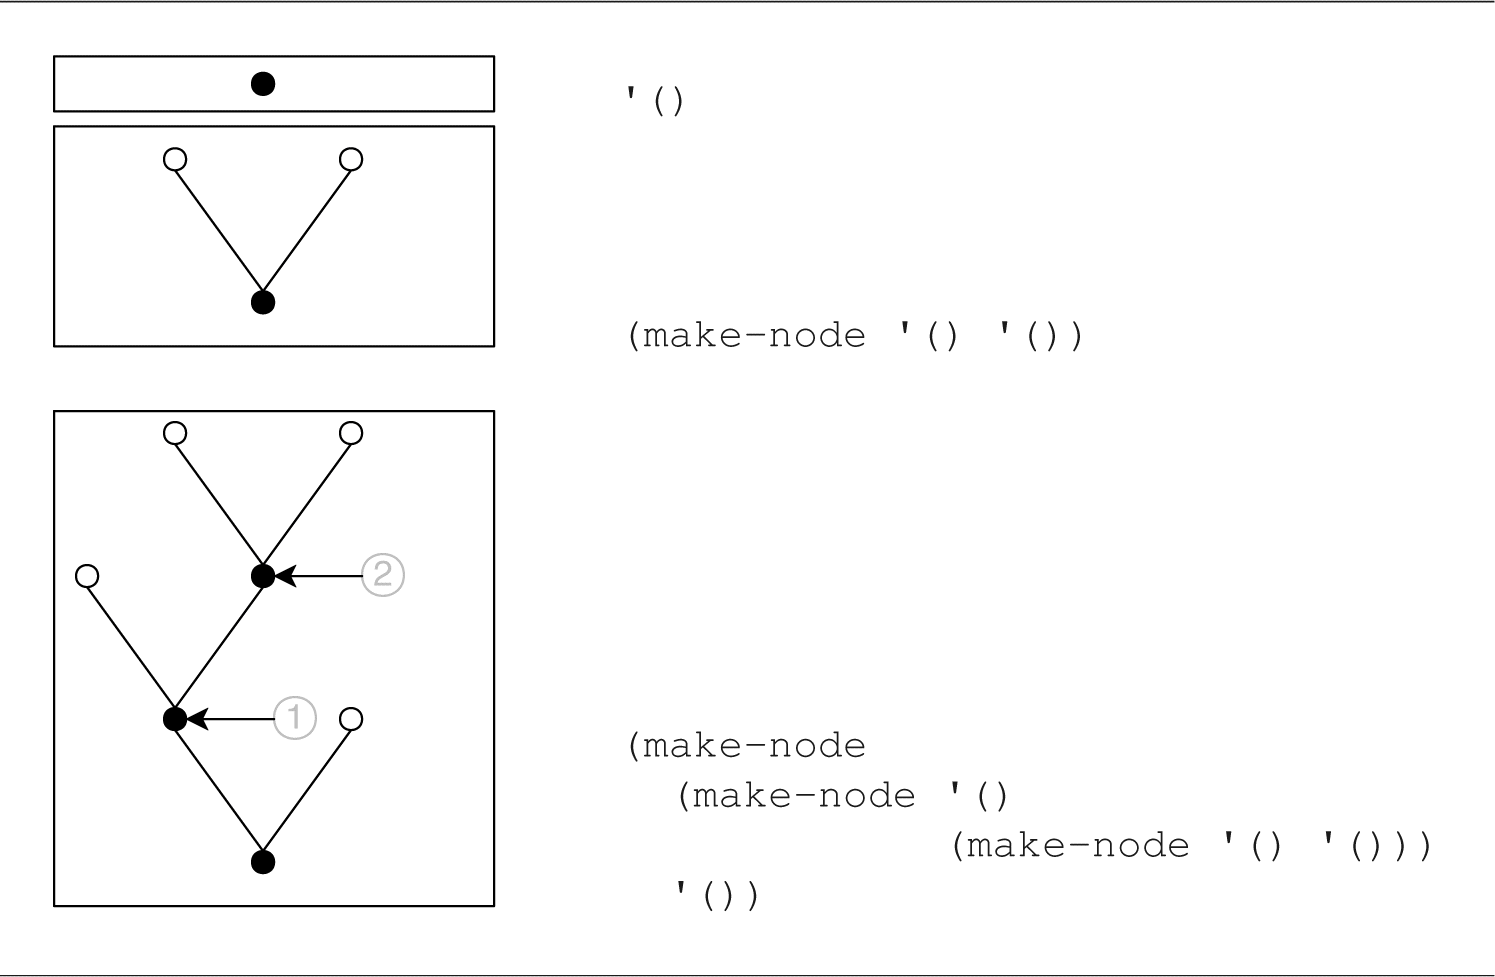
\includegraphics[width=0.85\textwidth]{images/00741.png}
  \caption{若干简化的二叉树结构示意}
  \label{fig:184}
\end{figure}

常规的结构化树高计算函数如下（这里将树高定义为从根节点到最深叶子节点的连接边数）：

\begin{lstlisting}[language=BSL]
; Tree -> N
; 计算二叉树的高度（边数）
(check-expect (height '()) 0)
(check-expect (height (make-node '() '())) 1)
(define (height abt)
  (cond
    [(empty? abt) 0]
    [else (+ 1 (max (height (node-left abt))
                    (height (node-right abt))))]))
\end{lstlisting}

为了将该函数改造为累加器风格，我们搭建标准的累加器模板。此时累加器所代表的上下文知识显而易见：
\begin{quote}
\textit{累加器 \code{a} 代表从整棵树的根节点 \code{abt0} 抵达当前正在遍历的子树 \code{abt} 所经过的边数（分支步数/当前深度）。}
\end{quote}

观察图 \ref{fig:184} 最底部的树：
\begin{enumerate}
  \item 若 \code{abt0} 为整棵树，而 \code{abt} 为带圆圈 1 所指向的子树，则此时累加器 \code{a} 的值必须为 1，因为从根节点到达它恰好迈出了一步；
  \item 同理，对于标号 2 的子树，累加器为 2，因为到达该位置走过了两步。
\end{enumerate}

不变量指示我们：初始深度为 0；每深入一层子树，更新操作为 \code{(add1 a)}；当触达空叶子 \code{\textquotesingle()} 时，当前累加器 \code{a} 就是从根节点沿该特定路径到达此叶子的深度，直接返回 \code{a}！

然而与前两个案例不同的是，二叉树包含左右两个递归分支。根据结构化设计配方，我们必须对左右子树返回的深度进行组合。由于树高定义为最大深度，我们使用 \code{max} 函数取两者较大值。图 \ref{fig:185} 给出了完整的实现。

\begin{figure}[htbp]
  \centering
\begin{lstlisting}[language=BSL, basicstyle=\scriptsize\ttfamily]
; Tree -> N
; measures the height of abt0
(check-expect (height.v2 example) 3)
(define (height.v2 abt0)
  (local (; Tree N -> N
          ; measures the height of abt
          ; accumulator a is the number of steps
          ; it takes to reach abt from abt0
          (define (height/a abt a)
            (cond
              [(empty? abt) a]
              [else
                (max
                  (height/a (node-left abt)  (+ a 1))
                  (height/a (node-right abt) (+ a 1)))])))
    (height/a abt0 0)))
\end{lstlisting}
  \caption{二叉树高度计算的累加器版本实现}
  \label{fig:185}
\end{figure}

\begin{notebox}[关于多累加器替代设计的探讨]
除了单纯累积当前路径的步数外，累加器函数还可以同时追踪迄今为止遭遇过的“全局最大高度”。这需要引入两个累加器参数：
\begin{itemize}
  \item 第一个累加器代表从 \code{abt0} 根节点到达当前节点 \code{abt} 的步数；
  \item 第二个累加器代表整棵树中严格位于当前子树 \code{abt} 左侧部分的最大高度。
\end{itemize}
其模板如下：
\begin{lstlisting}[language=BSL]
(define (height.v3 abt0)
  (local (
    (define (height/a abt path-len max-so-far)
      (cond
        [(empty? abt) (max path-len max-so-far)]
        [else
         (local ((define left-max
                   (height/a (node-left abt) (add1 path-len) max-so-far)))
           (height/a (node-right abt) (add1 path-len) left-max))])))
    (height/a abt0 0 0)))
\end{lstlisting}
这说明：\textbf{不同的累加器不变量会催生出不同的程序变体}。面对复杂方案，务必以设计依据与基准测试结果作为选型评判的标准。
\end{notebox}

\begin{exercise}{补全双累加器版本的 height.v3}{498}
完成 \code{height.v3} 的设计与全面测试。\textbf{提示}：仔细考查图 \ref{fig:184} 最底部的二叉树，在遍历标号为 1 的子树时，其左侧没有子树；而对于标号为 2 的子树，其左侧存在一条深度为 2 的完整路径。
\end{exercise}

\begin{exercise}{设计列表乘积 product 的累加器版本}{499}
设计计算数字列表中所有数值连乘积的累加器函数 \code{product.v2}。在表述完累加器不变量后，请先停下来仔细推敲其严密性。该常规函数的复杂度为 $\mathcal{O}(n)$，累加器版本是否能改善这一渐近时间复杂度？
\end{exercise}

\begin{exercise}{列表长度函数 how-many 与调用栈空间分析}{500}
设计计算列表元素个数的累加器风格函数 \code{how-many.v2}，并写出其不变量。

\begin{notebox}[核心概念：尾递归与栈空间开销 (Tail Recursion \& Stack Space)]
当手工推导常规版本的 \code{(how-many some-list)} 时，在函数最终触及 \code{\textquotesingle()} 时，内部挂起了 $n$ 个尚未完成的 \code{add1} 加法计算。计算机科学家称该函数需要 $\mathcal{O}(n)$ 的\term{调用栈空间}（stack space）来保存这些挂起的延时计算上下文。

而在累加器风格的 \code{how-many.v2} 中，递归调用发生在函数的最外层尾部，不再遗留任何后续计算（这称为\term{尾递归}，Tail Recursion）。现代编译器能够将这种尾递归自动优化为原地循环更新，从而将空间复杂度从 $\mathcal{O}(n)$ 大幅优化至 $\mathcal{O}(1)$ 常数空间！
\end{notebox}
\end{exercise}

\begin{exercise}{无加号累加计算 add-to-pi}{501}
设计累加器风格的 \code{add-to-pi} 函数。原函数通过递减自然数并不使用加号 \code{+} 来计算 $n + \pi$：
\begin{lstlisting}[language=BSL]
; N -> Number
; 在不使用 + 的前提下计算 n + pi
(check-within (add-to-pi 2) (+ 2 pi) 0.001)
(define (add-to-pi n)
  (cond
    [(zero? n) pi]
    [else (add1 (add-to-pi (sub1 n)))]))
\end{lstlisting}
写出累加器不变量并完成函数设计。
\end{exercise}

\begin{exercise}{构造回文列表 palindrome：四次遍历 vs 单次遍历}{502}
设计函数 \code{palindrome}，接收一个非空列表，并通过围绕最后一个元素镜像反转来构建回文。例如，当输入为 \code{(explode "abc")} 时，产生 \code{(explode "abcba")}。

\textbf{提示}：利用已有函数的组合解法如下：
\begin{lstlisting}[language=BSL]
(define (palindrome s0)
  (append (all-but-last s0)
          (list (last s0))
          (reverse (all-but-last s0))))
\end{lstlisting}
该组合方案需要遍历输入列表多达 4 次！请运用累加器配方设计一个\textbf{仅需单次遍历}即可直接生成目标回文列表的高效版本。
\end{exercise}

\begin{exercise}{矩阵行轮转选主元 rotate 与消除 append 性能隐患}{503}
第 28 章高斯消元法中需要对矩阵进行行轮转（选主元），直到首行首元素非零：
\begin{lstlisting}[language=BSL]
(define (rotate M)
  (cond
    [(and (cons? M) (not (= (first (first M)) 0))) M]
    [else (rotate (append (rest M) (list (first M))))]))
\end{lstlisting}
该生成型递归每次遇到 0 都会调用 \code{append}，导致大量的全新中间列表被创建并丢弃。当矩阵包含 5000 行且仅最后一行非零时，性能将极度恶化。

请使用结构型递归搭配累加器重新设计 \code{rotate}，使用累加器暂存那些首元素为 0 的行，彻底消除递归调用中反复调用 \code{append} 的性能瓶颈。
\end{exercise}

\begin{exercise}{将数字列表转为十进制数 to10}{504}
设计函数 \code{to10}。它接收一个数字列表，产生对应的十进制整数。列表中第一个元素是最高有效位。例如，应用于 \code{'(1 0 2)} 时，输出 102。利用领域知识：$1 \cdot 10^2 + 0 \cdot 10^1 + 2 \cdot 10^0 = ((1 \cdot 10 + 0) \cdot 10) + 2$ 提炼累加器不变量。
\end{exercise}

\begin{exercise}{质数判定函数 is-prime}{505}
设计函数 \code{is-prime}，输入一个大于 1 的自然数，当且仅当其为质数时返回 \code{\#true}。利用领域知识：一个数 $n$ 若不能被 $2$ 到 $n-1$ 之间的任何整数整除，则其为质数。分析为什么该函数的自顶向下递归必然面临“丢失原始输入 $n$”的问题，并运用累加器实现它。
\end{exercise}

\begin{notebox}[警惕思维定势：累加器并不总是更快！]
初学累加器的程序员容易产生一种刻板偏见，误以为累加器版本永远比常规递归版本快。然而实测表明，在特定运算和特定数据表示下，某些累加器函数（如阶乘函数在特定数值类型下的逆序计算）反而可能比常规版本慢。切勿盲从偏见，在软件工程实践中务必以严谨的性能基准测试数据说话！
\end{notebox}

\begin{exercise}{设计累加器版本的 map}{506}
为基础抽象函数 \code{map} 设计一个纯累加器风格的实现版本 \code{my-map}。
\end{exercise}

\begin{exercise}{从 foldr、reverse 深入理解 foldl 的本质}{507}
第 16 章曾指出，在结构化范式下，\code{foldl} 可以表达为先反转列表再调用 \code{foldr}。但一旦引入累加器，遍历列表的求值顺序天然被颠倒为从左向右！
\begin{enumerate}
  \item 为 \code{fold/a} 制定准确的函数签名并阐述其累加器不变量；
  \item 使用累加器风格独立设计 \code{build-l*st} 函数，使其行为与标准库的 \code{build-list} 严格一致。
\end{enumerate}
\end{exercise}

\section{扩展项目：支持鼠标交互的图形文本编辑器}
\label{sec:ch32_4}

第 5.10 节引入了单行文本编辑器的概念，并在第 10.4 节将其数据结构从单纯字符串重构为两个 1String 字符列表。之前的版本支持键盘左右箭头移动光标与退格删除，但现代图形应用无一例外都支持\textbf{鼠标点击定位光标}。

在单行文本编辑器中，用户在窗口中点击坐标 $(x, y)$，本质上是希望将光标准确插入到 $x$ 坐标所在位置左右相邻的字符之间。本节借助累加器来高效实现这一鼠标导航功能。

回顾第 10.4 节中的核心定义：
\begin{lstlisting}[language=BSL]
(define FONT-SIZE 11)
(define FONT-COLOR "black")

; [List-of 1String] -> Image
; 将字符列表渲染为编辑器中的文本图像
(define (editor-text s)
  (text (implode s) FONT-SIZE FONT-COLOR))

(define-struct editor [pre post])
; An Editor is a structure:
;   (make-editor [List-of 1String] [List-of 1String])
; 解释：(reverse pre) 对应光标左侧文本，post 对应光标右侧文本
\end{lstlisting}

\begin{exercise}{基于常规结构型设计光标分割函数 split-structural}{508}
使用结构化设计配方设计函数 \code{split-structural}。该函数接收一个字符列表 \code{ed} 和鼠标点击的横坐标自然数 \code{x}，产生一个新的 \code{(make-editor p s)}，满足：
\begin{enumerate}
  \item \code{p} 与 \code{s} 拼接后正好还原完整的 \code{ed}；
  \item 渲染 \code{p} 的图像宽度 $\le x \le$ 渲染 \code{(append p (first s))} 的图像宽度。
\end{enumerate}
\end{exercise}

\begin{exercise}{使用累加器高效重构 split 并集成鼠标事件}{509}
在上一题中，结构化设计在递归寻找断点时，往往需要反复测量前缀并丢弃已经量测的后缀。运用累加器设计配方设计函数 \code{split}，在单次遍历中顺向累加已丈量前缀的图像宽度与字符列表。

完成后，将该函数接入第 10.4 节编辑器的 \code{big-bang} 鼠标处理句柄中，体验通过鼠标点击任意调整光标位置的交互效果！
\end{exercise}

\begin{exercise}{开发文本自动折行格式化工具 fmt}{510}
类 Unix 操作系统中内置了著名的 \code{fmt} 工具，它能够重新排版文本文件中的单词，使得输出文本的每一行都不超过最大行宽 $w$。

设计程序 \code{fmt}。它接收最大行宽自然数 $w$、输入文件名 \code{in-f} 和输出文件名 \code{out-f}。它从输入文件中读取单词列表，使用累加器按行宽限制依次汇聚单词组装成行，最终将规整排版后的文本写入目标文件。
\end{exercise}
